%%%%%%%%%%%%%%%%%%%%%%%%%%%%%%%%%%%%%%%%%%%%%%%%%%%%%%%%%%%%%%%%%%%%%%%%%%%%%%%%
%%%%%%%%%%%%%%%%%%   Vorlage für eine Abschlussarbeit   %%%%%%%%%%%%%%%%%%%%%%%%
%%%%%%%%%%%%%%%%%%%%%%%%%%%%%%%%%%%%%%%%%%%%%%%%%%%%%%%%%%%%%%%%%%%%%%%%%%%%%%%%

% Erstellt von Maximilian Nöthe, <maximilian.noethe@tu-dortmund.de>
% ausgelegt für lualatex und Biblatex mit biber

% Kompilieren mit
% lualatex dateiname.tex
% biber dateiname.bcf
% lualatex dateiname.tex
% lualatex dateiname.tex
% oder einfach mit:
% make

\documentclass[
  tucolor,
  BCOR=12mm,     % 12mm binding corrections, adjust to fit your binding
  parskip=half,  % new paragraphs start with half line vertical space
  open=any,      % chapters start on both odd and even pages
  cleardoublepage=plain,  % no header/footer on blank pages
]{tudothesis}

% \usepackage{geometry}
% \geometry{a4paper, margin=2.5cm, top=3.5cm}
% \usepackage[onehalfspacing]{setspace}

% Warning, if another latex run is needed
\usepackage[aux]{rerunfilecheck}

% just list chapters and sections in the toc, not subsections or smaller
\setcounter{tocdepth}{1}

%------------------------------------------------------------------------------
%------------------------------ Sprache und Schrift: --------------------------
%------------------------------------------------------------------------------
\usepackage{fontspec}
\defaultfontfeatures{Ligatures=TeX}  % -- becomes en-dash etc.

% german language
\usepackage{polyglossia}
\setdefaultlanguage{english}

% for german parts if needed
\setotherlanguages{german}

% intelligent quotation marks, language and nesting sensitive
\usepackage[autostyle]{csquotes}

% microtypographical features, makes the text look nicer on the small scale
\usepackage{microtype}

%------------------------------------------------------------------------------
%------------------------ Für die Matheumgebung--------------------------------
%------------------------------------------------------------------------------

\usepackage{amsmath}
\usepackage{amssymb}
\usepackage{mathtools}

% Enable Unicode-Math and follow the ISO-Standards for typesetting math
\usepackage[
  math-style=ISO,
  bold-style=ISO,
  sans-style=italic,
  nabla=upright,
  partial=upright,
]{unicode-math}
\setmathfont{Latin Modern Math}

% nice, small fracs for the text with \sfrac{}{}
\usepackage{xfrac}


%------------------------------------------------------------------------------
%---------------------------- Numbers and Units -------------------------------
%------------------------------------------------------------------------------

\usepackage[
  locale=DE,
  separate-uncertainty=true,
  per-mode=symbol-or-fraction,
]{siunitx}
\sisetup{math-micro=\text{µ},text-micro=µ}

%------------------------------------------------------------------------------
%-------------------------------- tables  -------------------------------------
%------------------------------------------------------------------------------

\usepackage{booktabs}       % stellt \toprule, \midrule, \bottomrule

%------------------------------------------------------------------------------
%-------------------------------- graphics -------------------------------------
%------------------------------------------------------------------------------

\usepackage{graphicx}
\usepackage{grffile}
\usepackage{subcaption}

% allow figures to be placed in the running text by default:
\usepackage{scrhack}
\usepackage{float}
\floatplacement{figure}{htbp}
\floatplacement{table}{htbp}

% keep figures and tables in the section
\usepackage[section, below]{placeins}


%------------------------------------------------------------------------------
%---------------------- customize list environments ---------------------------
%------------------------------------------------------------------------------

\usepackage{enumitem}

%------------------------------------------------------------------------------
%------------------------------ Bibliographie ---------------------------------
%------------------------------------------------------------------------------

\usepackage[
  backend=biber,   % use modern biber backend
  autolang=hyphen, % load hyphenation rules for if language of bibentry is not
                   % german, has to be loaded with \setotherlanguages
                   % in the references.bib use langid={en} for english sources
]{biblatex}
\addbibresource{references.bib}  % die Bibliographie einbinden
\DefineBibliographyStrings{german}{andothers = {{et\,al\adddot}}}

\usepackage[labelformat=simple]{subcaption}
\renewcommand\thesubfigure{(\alph{subfigure})}

%------------------------------------------------------------------------------
%------------------------------ Sonstiges: ------------------------------------
%------------------------------------------------------------------------------

\usepackage[pdfusetitle,unicode,linkbordercolor=tugreen]{hyperref}
\usepackage{bookmark}
\usepackage[shortcuts]{extdash}
\usepackage{blindtext}

%------------------------------------------------------------------------------
%-------------------------    Angaben zur Arbeit   ----------------------------
%------------------------------------------------------------------------------

\author{Kevin Sedlaczek}
\title{Analysis of the Crab Nebula using Photon Stream data collected by FACT}
\date{\today}
\birthplace{Dortmund}
\chair{Lehrstuhl für Experimentelle Physik Vb}
\division{Fakultät Physik}
\thesisclass{Master of Science}
\submissiondate{31. Dezember 2018}
\firstcorrector{Prof.~Dr.~Dr.~Wolfgang Rhode}
\secondcorrector{Prof.~Dr.~Zweitkorrekteur}

% tu logo on top of the titlepage
\titlehead{
\includegraphics[height=1.5cm]{logos/tu-logo.pdf}}

\begin{document}
\frontmatter
% \input{content/hints.tex}
\maketitle

% Gutachterseite
\makecorrectorpage

% hier beginnt der Vorspann, nummeriert in römischen Zahlen
\chapter{Abstract}

This work is investigating the novel data format \textit{Photon Stream} by
analyzing physics data of the Crab Nebula. \textcolor{red}{Nicht vollständig}
\\
\\
In dieser Arbeit wird das neuartige Datenformat \textit{Photon Stream} im
Zusammhang einer Analyse des Krebsnebels untersucht.

\tableofcontents

\mainmatter
% Hier beginnt der Inhalt mit Seite 1 in arabischen Ziffern
\chapter{Introduction}
\nocite{biblatex, siunitx, Hunter:2007}%
%
\begin{aquote}{\textit{Albert Einstein}}
\textsc{One cannot help but be in awe when he contemplates the mysteries of eternity, of life, of the marvelous structure of reality.}
\end{aquote}
In physics, the search for a fundamental understanding of reality is ubiquitous. The understanding of the universe we live in and the rules of nature has
led mankind to look for the things beyond earth. To understand what these rules
are, on earth and in the universe, is the goal of astrophysics. The electromagnetic radiation reaching the earth from space has opened the window to learn
about the universe beyond our planet. The discovery of this extraterrestrial
radiation by Victor Hess during his balloon flights around \num{100} years ago in \num{1912}~\cite{Hess} marks the beginning of the observation of this radiation.
Today we know that the electromagnetic radiation spans a very large range of
frequencies and reaches up to the highest energies ever measured \cite{source}.
The different energy ranges of cosmic radiation caused the development of a
variety of different telescopes, specialized on certain frequency bands. On
ground, only visible light and radio waves from space can be observed directly,
due to the absorption of Earth's atmosphere. Therefore, large optical and radio
telescopes have been built to observe stars, galaxies and other objects from
Earth. Of course, the atmosphere still has an impact on the observations, so
there are optical telescopes in space as well, like the Hubble Space
Telescope~\cite{hubble}, observing infra-red to ultra-violett light. However,
some telescopes take advantage of the atmosphere's impact, by using it as a
giant detector volume. Among these telescopes are the Imaging Air Cherenkov
Telescopes (IACT), observing cosmic rays via their interaction products. This
work is based on the observations of such a telescope, described in
\autoref{ch:fact}. The development and advancement of new telescopes continues
today, as the currently constructed Cherenkov Telescope Array CTA~\cite{cta}
will yield unprecedented accuracy and sensitivity among IACTs.
Among the goals of astrophysics are not only the understanding of the
structures of the universe, but also the very elementary interactions of
particles within the sources of this radiation. The very first hints for the
existance and characteristics of dark matter~\cite{zwicky}, a supposed
elementary particle for instance originate from the field of astrophysics.
This work focuses on the rather technical aspect of a new data representation
and its implications for IACT analyses, by analyzing a data set of this new data
format for the first time.

\chapter{Imaging Air Cherenkov Astronomy}
\label{ch:iact}
%
\begin{figure}[H]
  \centering
  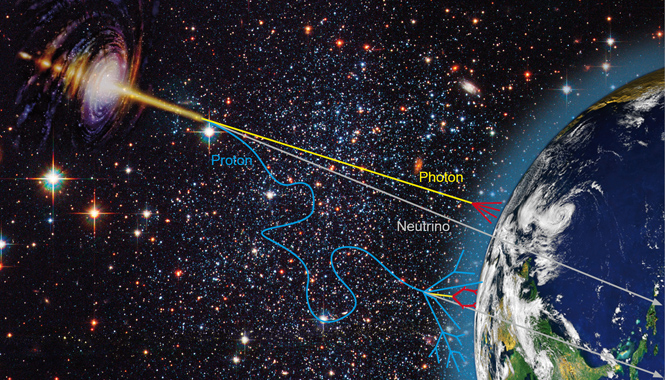
\includegraphics[width=0.95\textwidth]{Plots/cosmic_rays.jpg}
  \caption{Different constituents of the cosmic rays reaching earth \cite{cosmic-rays}. There are three different particle types of cosmic rays that can be used for astronomy. The uncharged and very light neutrinos (white) barely interact with anything on their way through the universe. Thus, they give strong hints on their origin, but are very hard to detect as well. The charged particles such as protons or ionized atoms (blue) are deflected by magnetic fields and therefore lose any direction information. Lastly, cosmic gamma-rays (yellow), massless uncharged photons, are emitted through various processes and from different sources such as active galctic nuclei. They are not deflected much and are the main signal for Cherenkov astronomy.}
  \label{fig:rays}
\end{figure}
%
The atmosphere of earth is continously penetrated by radiation from different
sources within our universe. This cosmic radiation is made up of different types
of particles, interacting with the atmosphere in various ways. There are
charged protons and the uncharged neutrinos and photons (gamma rays). Neutrinos
are uncharged, very light fermions, that interact very weakly and are not
detectable by optical telescopes at all. Protons make up the largest number of
particles reaching earths atmosphere. Due to their electric charge, they are
deflected by magnetic fields and therefore lose information on their origin on
the way to earth, making them unsuitable for Cherenkov astronomy.
%
\section{Cosmic Gamma-Rays}
%
Cosmic gamma-rays are photons with a very high energy, originating from bright
sources such as active galactic nuclei or nebulae. When such particles intersect
with earth's atmosphere, they create new particles moving faster than light
within that atmosphere due to their high energy. Particles moving at such
speeds through a medium cause, among the creation of other particles, the
emission of bluish photons, the Cherenkov-light.
Cherenkov-light is emitted by the medium directly from the moving particle
within a specific angle towards the direction of movement of that primary
particle.
%
\begin{equation}
    \cos(\vartheta) = \frac{1}{n\beta}
    \label{eq:angle_cherenkov}
\end{equation}
%
As \autoref{eq:angle_cherenkov} shows, this angle depends on the index of
refraction $n$ of the medium and the particle's velocity. Due to this emission
angle the light traverses the medium in a cone-shape, when being described from
earth's point of view. By the time it is reaching the ground it thus
illuminates an elliptical area of about $\SI{200}{\meter}$ diameter, depending
on the height of interaction and the primary particle's energy.
This already implicates that the light, although a secondary product of the
cosmic gamma-ray, can be used to reconstruct physical properties of
said gamma-ray. To do so, the flashes of the Cherenkov-light need to
be captured by cameras capable of filming very short time scales (about
$\SI{e-9}{\second}$).

\section{Imaging Air Cherenkov Telescopes}

Imaging Air Cherenkov Telescopes (IACTs) are using videos of this light, to
reconstruct properties of the incident cosmic radiation above
$\SI{100}{\giga\electronvolt}$, by analyzing the spatial geometry of the
measured pictures.

The three properties of interest for each event are:
%
\begin{description}[labelsep=1em]
  \item[source position]{the position of the source of the primary particle on the sky}
  \item[particle type]{the distinction between cosmic gamma rays and other particles like protons or secondary particles like muons}
  \item[particle energy]{the energy of the primary gamma-ray}
\end{description}
%
This means that the task is to resolve single incoming cosmic gamma rays and
reconstruct these properties. By doing so, the atmosphere is used as a very
wide spread detector. When trying to avoid any interactions of the incident
particles and measuring their properties directly in a specifically prepared
detector material, one eventuually has to leave earth's atmosphere. Such direct
measurements are carried out in earth's orbit, outside its atmosphere.
Detectors like the Fermi Large-Area-Telescope \cite{fermiLAT} (Fermi LAT) are satellites
carrying their own detectors for the necessary measurements. They consist of
interaction volumes taking over what the atmosphere does to intersecting cosmic
rays: particles like gamma rays interact with the material, creating new
particles by losing energy, which then continue to do so in particle cascades
until the energy has spread to a certain amount. This process is called
shower (or air-shower, depending on the medium of interaction). The
characteristics of these interactions and the produced particles strongly
depend on the properties of the incident particle, such as energy and particle
type. There are particles that mainly interact via the electromagnetic force.
Such showers are called electromagnetic showers. They are usually initiated by
photons or electrons and mainly consist of light, charged fermions like electrons or
muons and photons or light, charged bosons like pions. Showers initiated by
hadronic cosmic rays like protons show different kinds of interactions, also
resulting in different spatial topologies. The momentum perpendicular to the
primary particle's trajectory is bigger, giving the shower a wider spread of
secondary particles. This is the main characteristic to distinguish hadronic
showers, resembling the main background within the measurements (apart from
muons) from signal gamma rays. When a proton interacts with a
nucleus within the atmosphere or a dedicated detector material, a lot of
different particles can be created. Heavier hadrons usually quickly decay into
the lightest ones which are protons for the class of baryons as well as pions
for the class of mesons. The pions mainly decay into muons, which eventually
yield electrons and neutrinos. During all those interactions photons and
electrons and their anti-particles as well as neutrinos are created. The
neutrinos very rarely contribute to any interactions after their creation,
whereas electrons can interact with photons, emit or absorb them or annihilate
to such.

\begin{figure}
  \centering
  \begin{subfigure}{0.475\textwidth}
    \centering
    \includegraphics[width=0.85\textwidth]{example-image-a}
    \label{fig:proton}
  \end{subfigure}
  \begin{subfigure}{0.475\textwidth}
    \centering
    \includegraphics[width=0.85\textwidth]{example-image-b}
    \label{fig:gamma}
  \end{subfigure}
  \caption{Simple sketch of the two different shower types.}
  \label{fig:shower}
\end{figure}

Considering this, the higher the energy of the incident particle the more
energy is available for the resulting shower. Thus, the size of these showers
is expected to strongly correlate with the energy. But, to register a cosmic
ray, there has to be interaction first. The effective area of the telescope
is mainly determined by the interactions that can be covered by the sensors. So
bringing up a detector to earth's orbit strongly limits the sensored
interaction material, which already highlights the disadvantage of satellite
telescopes: the amount of interaction material is strongly limited and the
measurement is strongly dependent on that quantity. Direct measurements, e.g.
can derive the direction of cosmic rays by reconstructing the interactions of
the cosmic ray itself inside the tracker volume, rather than secondary
particles. They also give the possibility to measure the energy by counting the
energy depositions within a well calibrated and understood calorimeter, as well
as the particle type. But the strong limitations on size and weight confine the
effective areas of such telescopes very strictly. Thus, detectors in space are
usually unable to resolve time structures of events, but are well suited for
static and wide field-of-view surveys with large exposure times. Since the
abundance of cosmic rays is dependent on the energy and high energy cosmic rays
are much less likely to appear, such detectors are rather suited for the lower
energies.

So there are quite some disadvantages that direct measurements have over
indirect measurements and vice versa. Of course, using the atmosphere means
using a detector undergoing strong, uncontrollable fluctuations in all its
properties. It also means using a detector that is bigger than anything
man-build and readily available. Good understanding of these fluctuations and
the respective modelling is crucial for the analysis of the data.

High energy cosmic particles interacting with the earth's atmosphere generate
showers as described above in a highly boosted way. The secondary particles
therefore continue their trajectories almost parallel to the incident particle.
The spatial distribution of the shower again depends on the energy of the
cosmic ray, ranging from several kilometers to showers not reaching their
climax before hitting the ground. IACTs record the Cherenkov photons of the
showers from energies of about $\SI{100}{\giga\electronvolt}$ to the highest
energies of the cosmic spectrum. But since the cosmic ray energy spectrum
rapidly decreases at high energies, the majority of the recorded events
resemble the lower energy limit of the telescopes.

\chapter{The First G-APD Cherenkov Telescope}
%
\begin{figure}
  \centering
  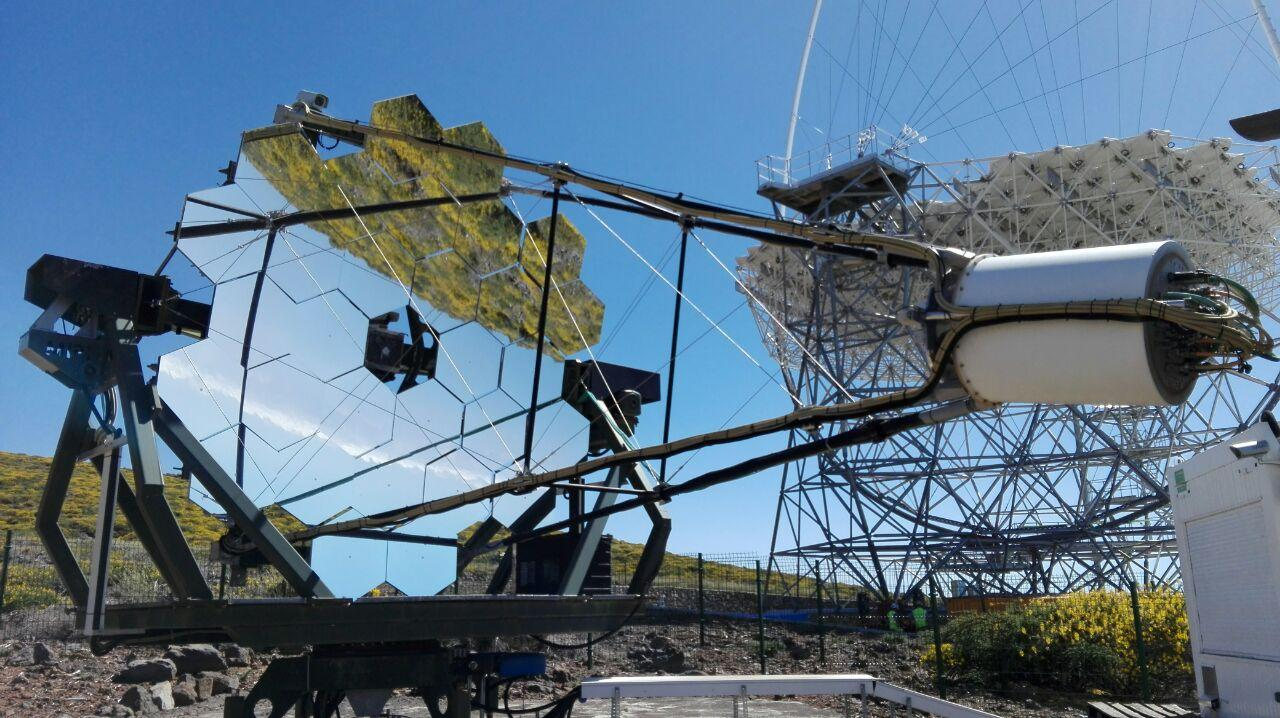
\includegraphics[width=\textwidth]{Plots/fact.jpg}
  \label{fig:fact}
  \caption{The First G-APD Cherenkov Telescope on the Observatory on the Roque des los Muchachos on the island of La Palma. Image courtesy of Kevin Schmidt.}
\end{figure}
%
The First G-APD Cherenkov Telescope \cite{FACT-Design} (FACT) is an IACT
protoype located $\SI{2200}{\metre}$ above sea-level on the Canary island of La
Palma. It measures air-shower-photons from cosmic gamma-rays with energies from
several hundred GeV up to about $\SI{10}{\tera\electronvolt}$. FACT uses a
segmented imaging-reflector with a $\SI{9.5}{\meter\squared}$ aperture and
$\SI{4.889}{\meter}$ focal-length. Apart from monitoring bright sources of
cosmic gamma-rays, like Markarian 421 and Markarian 501, FACT is used for
demonstrating and testing the usage of new technologies in the field of IACTs.

Giving it its name, FACT uses a novel kind of detector made of so called
Geiger-mode avalanche photomultipliers (GAPD). These photomultipliers make up
the 1440 pixels of Silicon-Photo-Multipliers (SiPM), FACT uses to sense
photons. Each pixel yields about $\SI{0.1}{\degree}$ field-of-view, giving FACT
a total field-of-view of $\SI{4.5}{\degree}$. Using SiPMs instead of
Photo-Multiplier-Tubes (PMTs) differentiates FACT from other IACTs and gives it
special possibilities. SIPMs are very robust, compared to PMTs and can operate
in brighter light. This makes continuos observations even during bright moon
possible. The SIPMs furthermore have a high photon detection efficiency and
therefore the potential to replace PMTs in IACTs. FACT is sampling recorded
events with a frequency of $\SI{2}{\giga\hertz}$, giving it a very good time
resolution. With these assets, FACT is well suited for long-term monitoring of
sources, finding flares and informing the astronomic community of such.

\chapter{Representing IACT data}
%
IACTs aim at reconstructing the energy, source position and particle type of
cosmic rays via their Cherenkov-light. The Cherenkov-light flashes that are
only nano seconds in duration are measured and can be separated from background
light from stars or ambient light by their brightness and topology within the
camera image. There are different ways to represent air shower data. FACT uses
the so called main-pulse representation, whereas this work focuses on a novel
data format, both of which are described in the following chapter.

\section{The Main-Pulse representation}
%
Data taken by an Imaging-Air-Cherenkov-Telescope
(IACT), like FACT, is usually represented in so called time series.
These time series owe their name to the fact that they represent voltages at the photosensors over time. Within these time series lie so called main-pulses that represent the increased voltage that a charge deposition of an air-shower causes. So by looking for those main-pulses shower events can be found upon the detector noise and ambient light in the camera. Of course, the main-pulses consist of multiple photon signals and noise superposed over time, but in this state they are electric pulses representing the response of very specific hardware. So rather than measuring physical properties, this means that the charge deposit has to be interpretated to be transferred into physics observables, independant of these specifics \textbf{[which ones?]}. Such interpretations always include assumptions of physical and technical kinds. By integrating the charge in one pixel an equivalent of a photon count can be obtained, called the \textit{photon equivalent} (PE). So the first observable in this representation is the PE which corresponds to the best estimate of the number of photons measured per pixel. The photon counts are spatially located by the corresponding pixel they are assigned to. The 1440 pixels of FACT are the determining grid that yield the spatial coordinates of every shower event.

The second observable is the time. When the telescope is triggered and records
data the arrival time of the event is measured via the time information within
the time series. From the time series a quantized timing information per pixel
can be developed by dividing the event into time slices. From this the arrival
time of the photons per pixel can be calculated by averaging. Thus, the arrival
times $t$ per pixel are the second observable of the main-pulse event
representation, besides the photon-equivalents.

\begin{figure}
  \begin{subfigure}{0.475\textwidth}
    \includegraphics[width=1.1\textwidth, page=40]{Plots/cleaning_facttools_pe_20131104_162.pdf}
  \end{subfigure}
  \begin{subfigure}{0.475\textwidth}
    \includegraphics[width=1.1\textwidth, page=40]{Plots/cleaning_facttools_arrival_times_20131104_162.pdf}
  \end{subfigure}
  \caption{The measured observables of the main-pulse representation are shown as scatter plots within the pixels. On the left the distribution of photon-equivalents $c$ of a typical shower event (Crab observation on November, 4th 2013, run 162, event 80) is shown. On the right the arrival times of that event's photons with respect to the mean arrival time in ns are displayed.}
  \label{fig:mainpulse}
\end{figure}

\section{The PhotonStream representation}

The Photonstream representation aims at creating a data format consisting of photons by storing their observed physical properties. So from the measured time series single photons are extracted instead of deriving photon counts in pixels. Each of these photons is assigned an arrival time and pixel, creating a list of arrival times per photon for each pixel. By doing so, a 3-dimensional data set is created, which can be represented in form of so called point clouds (\autoref{fig:event}).
%
\begin{figure}
  \centering
  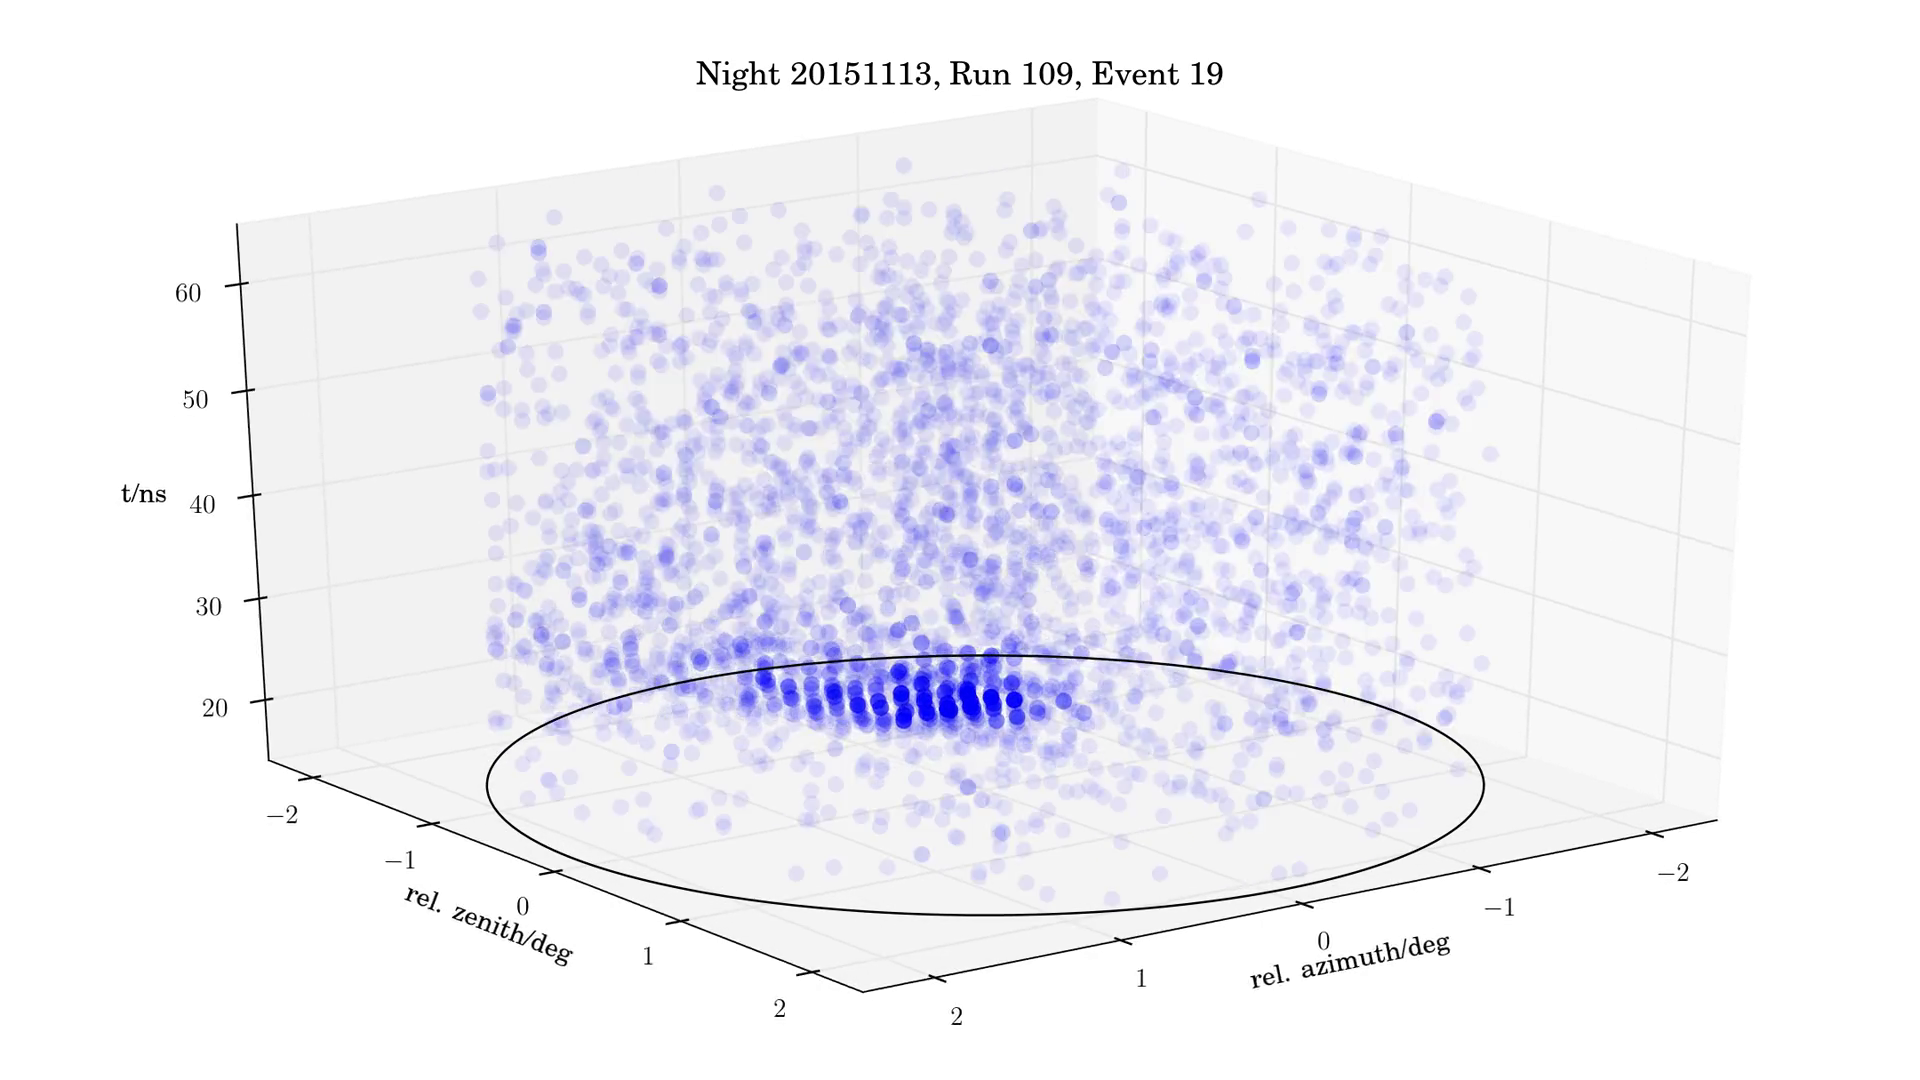
\includegraphics[width=1.1\textwidth]{Plots/event2.png}
  \caption{Uncleaned event represented by the 3-dimensional point cloud of the Photonstream. Every blue sphere represents a measured photon in the corresponding time slice and pixel.}
  \label{fig:event}
\end{figure}

\chapter{Analysis chain}
%

\section{Image Cleaning on the PhotonStream}
%
As pointed out in \autoref{ch:iact} the Cherenkov-light of air-showers shows a
very specific topology. The emitted photons are coherent in space and time:
they originate from a single very high energetic and therefore very fast
primary particle and thus appear in a very brief time window of a few
nanoseconds. Furthermore, the characteristic Cherenkov-angle under which the
light is emitted, creates a light cone, which, when projected to the
$x$-$y$-plane of the camera causes the specific elliptical shape. Both of these
topological features are mandated by the physical process and can therefore be
unrestrictedly used for the cleaning. Background events like ambient light or
starlight don't show these characteristics and tend to appear randomly.

The threedimensional $xyt$-representation of the PhotonStream's point-cloud
quantifies photons with exactly those three observables. Thus, a cleaning
within the threedimensional space-time can heavily use the known topology.
Within the point-cloud, an air-shower will appear as a very dense cluster of
photons, surrounded by a merely isotropic distribution of background photons.
These characteristics of shower events in the PhotonStream representation
naturally suggest a density-based clustering algorithm as the cleaning method
of choice. The two challenges at hand are the choice of a suited algorithm and
a well defined metric to make the threedimensional spacetime usable.

\subsection{Air-showers in the point-cloud}
%
The threedimensional spacetime of the PhotonStream and its representation as a
point-cloud eventually mixes spatial dimensions with time. While this is
physically motivated, defining distances in such a space is not trivial. They
are highly dependent on the chosen metric, which defines how time correspondsto
space. This already implies that the choice of metric contains certain
assumptions and can be adapted to specific preferences. The essential parameter
is the factor $\alpha$, which transfers time to space and vice versa:
%
\begin{equation}
  c_{t} = \alpha \cdot t \, .
  \label{eq:metric}
\end{equation}
%
The choice of this parameter e.g. gives the possibility to prefer spatial
distance over timing information, or the opposite. The spacetime of the
point-cloud is quantized in all its three dimensions: the pixels of the camera
define the spatial grid, whereas the time slices, each event is binned to, do so
for the timing information. When trying to separate air-showers from
background via the density of the shower's photons, the distance plays the
essential role. The natural way to equalize between space and time is to adapt
to the photon distribution of a typical air-shower along each axis. So, by
choosing
%
\begin{equation}
  \alpha = 0.35\cdot10^9\,\si{\degree\per\second}
\end{equation}
%
the one-dimensional density distribution of photons along the coordinates
$c_x$, $c_y$ and $c_t$ is the same. With this metric, the distance between two
photons $a$ and $b$ is defined as
%
\begin{equation}
  d_{a,b} = \sqrt{(c_x^a - c_x^b)^2 + (c_y^a - c_y^b)^2 + (c_t^a - c_t^b)^2}
\end{equation}

The twodimensional projections of the point-cloud within this metric are shown
in \autoref{fig:pc} for an example air-shower event. With the calculated
degree-equivalent of time the air-shower shows a similar distribution in
each dimension.
%
\begin{figure}[H]
  \centering
  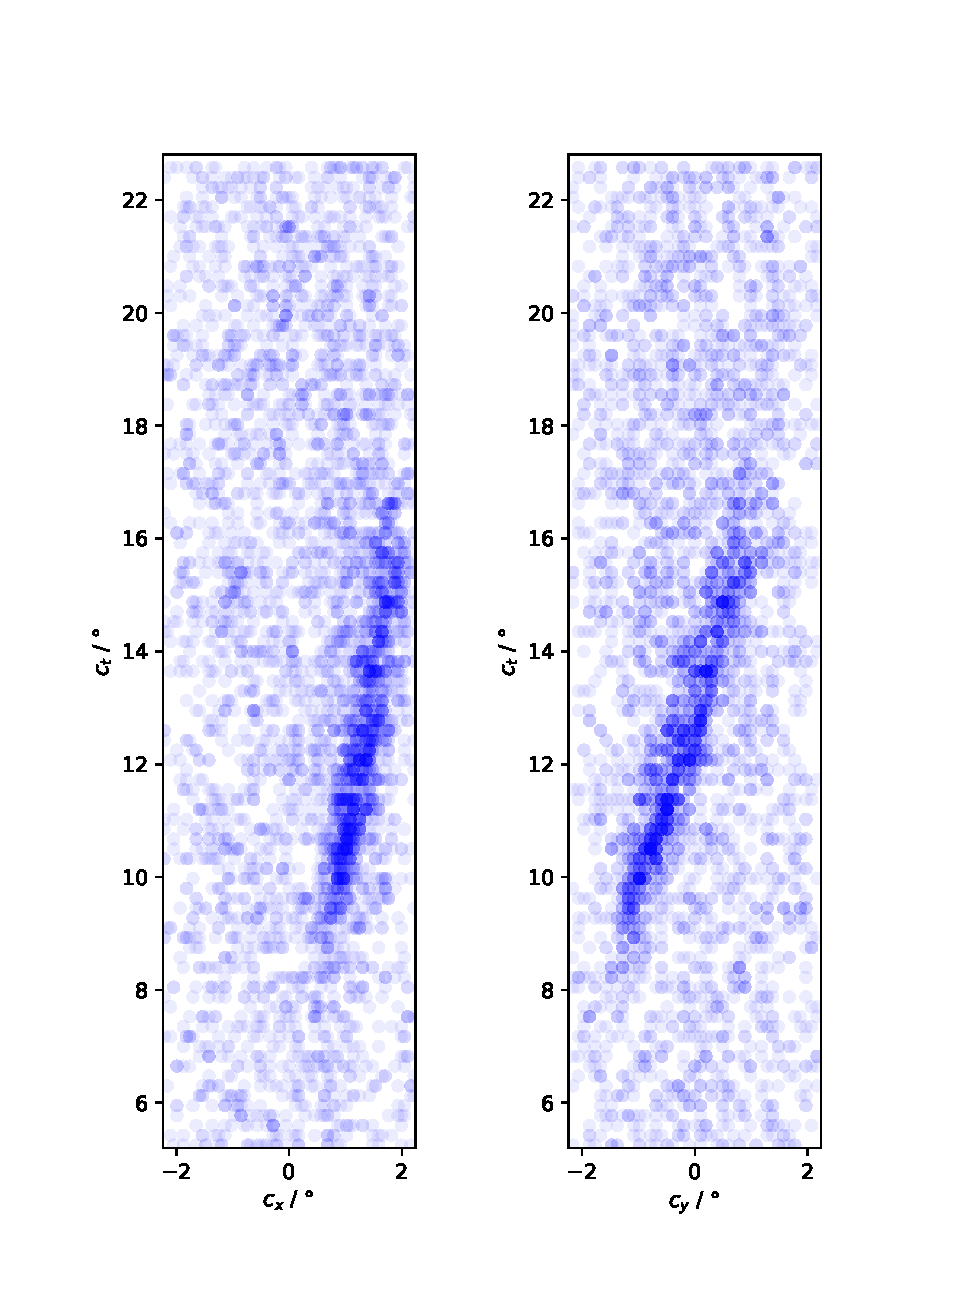
\includegraphics[width=0.6\textwidth, angle=-90]{Plots/point_cloud.pdf}
  \caption{Twodimensional projections of the point-cloud using the metric described above.}
  \label{fig:pc}
\end{figure}
%

\subsection{Density-based Clustering with DBSCAN}
%
To find clusters of photons within the space described above, the PhotonStream
uses the \textit{density-based algorithm for discovering clusters with noise}
(DBSCAN) \cite{DBSCAN}. The DBSCAN is well suited for finding air-showers with the
PhotonStream's observables, when choosing the right parameter set for the algorithm. This
algorithm either assigns each extracted photon to one of potentially multiple
clusters or identifies it as a night-sky-background photon. There are no
assumptions on the shape, location or number of the clusters. The algorithm is
characterized by only two parameters.
%
\begin{description}[align=right]
  \item[m] the minimum number of photons to make up a cluster
  \item[$\symbf{\varepsilon}$] the maximum distance between two photons to be considered dense
\end{description}
%
These two parameters represent the specific topology of the air-shower events
by giving limits on typical shower sizes and spreads in spacetime. For
air-shower events recorded by FACT the best choice was found to be $m = 20$ and
$\varepsilon = \SI{0.45}{\degree}$. So, to survive the cleaning, every found
cluster must at least contain 20 photons within a maximum distance of
$\SI{0.45}{\degree}$ to the respective closest photon. The algorithm determines
the clusters by iterating over the photons in 4 steps:
%
\begin{enumerate}
  \item loop over photons until a dense region with at least $m$ photons is found
  \item add photons to the newly found cluster that are within distance $\varepsilon$ or connected via a chain of dense photons
  \item if nothing to add to cluster restart 1. with leftover photons
  \item mark all photons not assigned to any dense cluster as night-sky-background
\end{enumerate}
%
This way every photon is either belonging to a cluster of an air-shower, or
discarded as background. This determination is taking place in the whole space
of observables the whole time. There are no intermediate steps, only taking
single observables into account, which very much represents a way to find
air-showers in a space well suited for describing them. Furthermore, this way
single photons are selected rather than specific pixels. When expecting
background photons also within signal pixels, this should yield a cleaned image,
closer to the true air-shower image.
%
\begin{figure}
  \begin{subfigure}{0.5\textwidth}
    \centering
    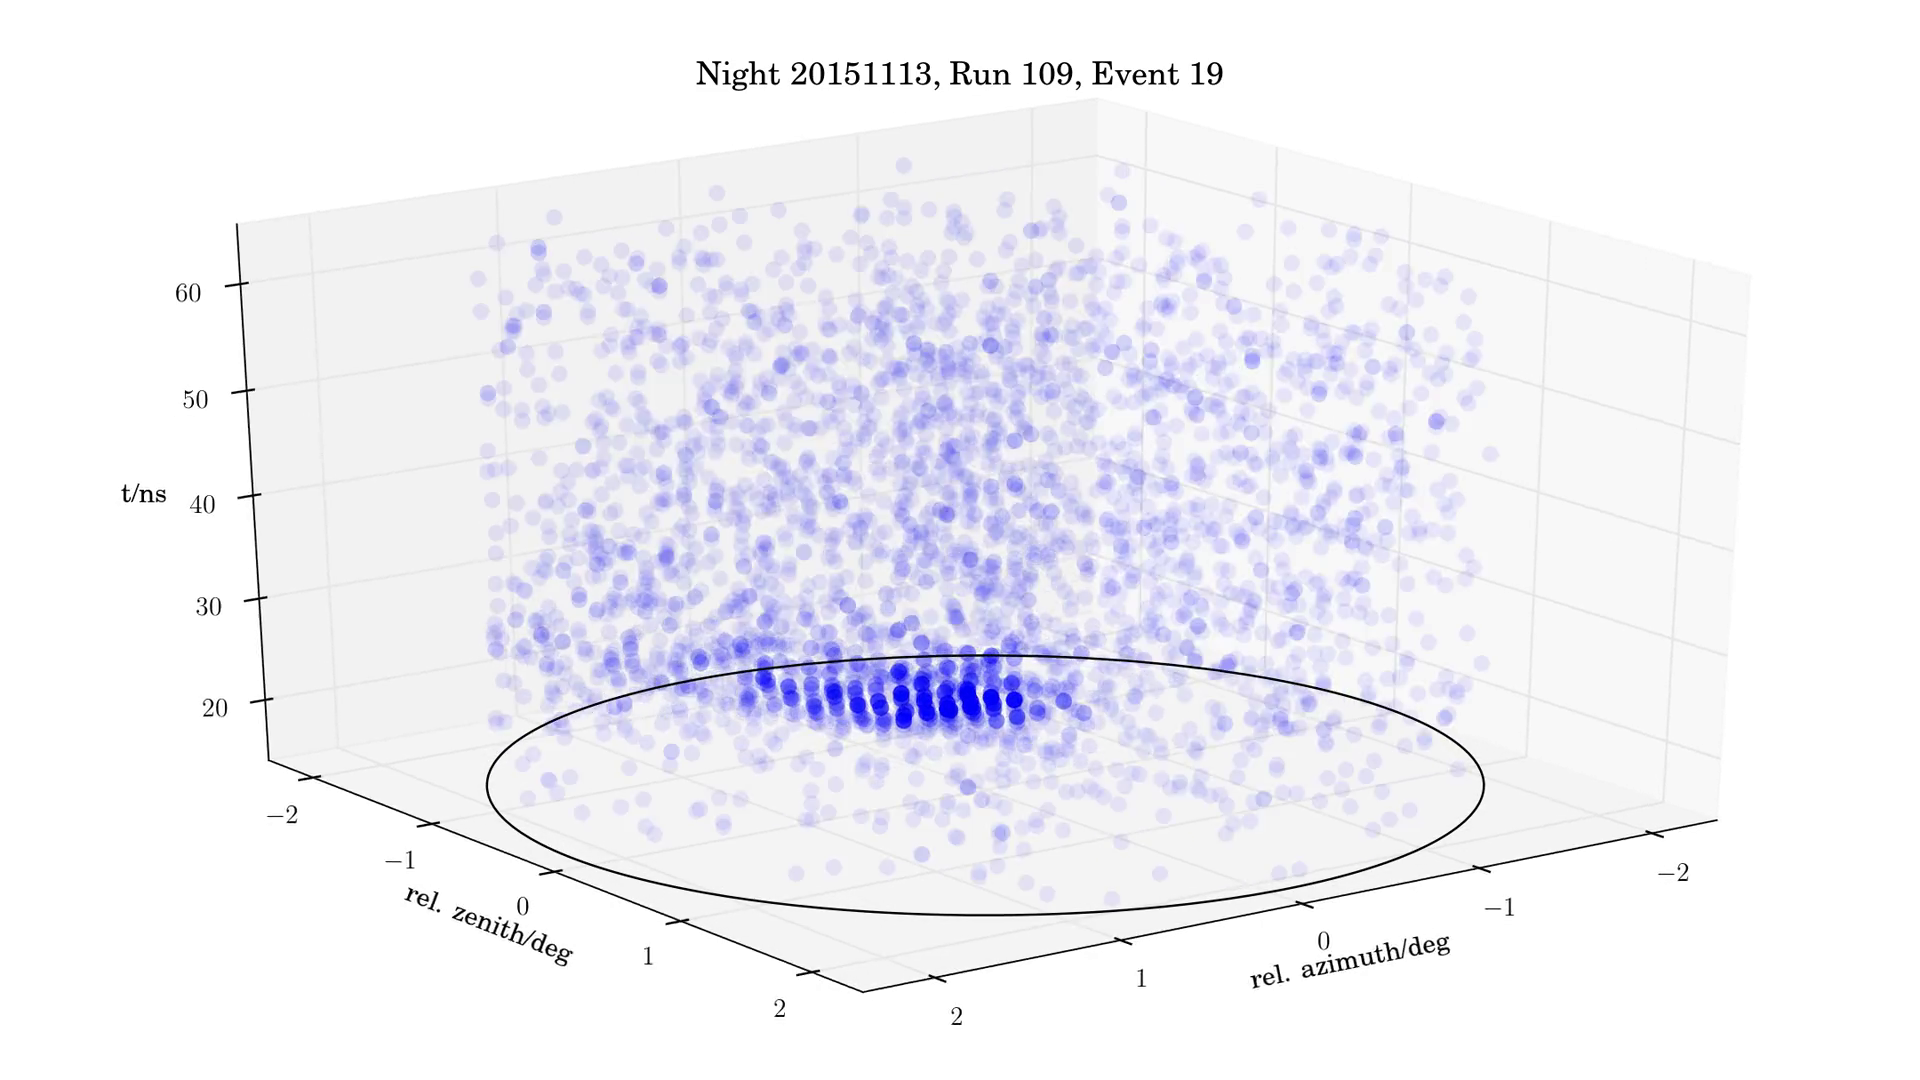
\includegraphics[width=1.1\textwidth]{Plots/event2.png}
  \end{subfigure}
  \begin{subfigure}{0.5\textwidth}
    \centering
    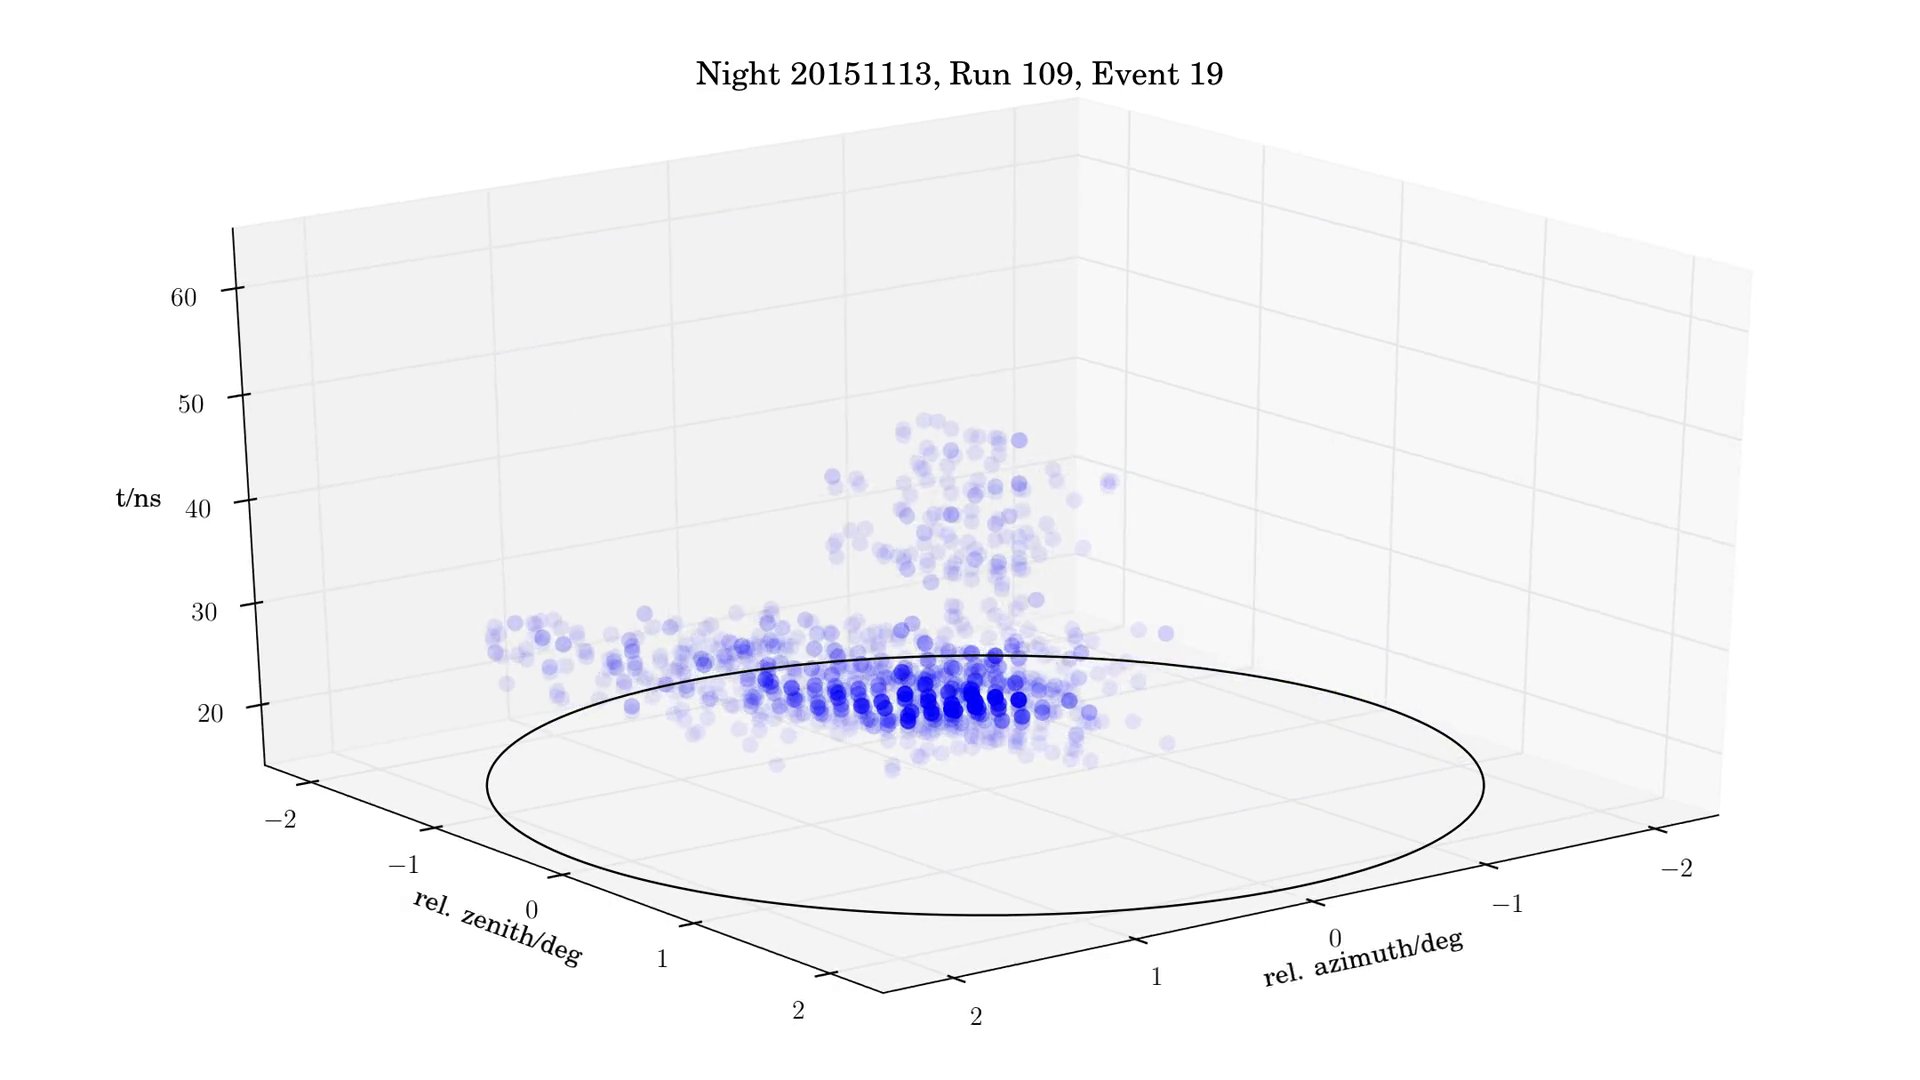
\includegraphics[width=1.1\textwidth]{Plots/event1.png}
  \end{subfigure}
  \caption{Event represented by the 3-dimensional point cloud of the Photonstream. Every blue sphere represents a measured photon in the corresponding time slice and pixel. The right figure shows the remaining photons after cleaning.}
  \label{fig:event}
\end{figure}
%

\section{Parametrization of Events}
%
For the classical analysis the detected images need to be parametrized. The
learning algorithms work with specific features rather than the whole image,
although there are indeed ways to analyze single pixels.

The parametrization that is most frequently chosen for IACT data is based on
the one proposed by Hillas~\cite{Hillas}. It operates on the two dimensional
images recorded by the cameras, calculating features of the air-shower pixels.
In the original publication these features were used to successfully analyze
images on a 37-pixels camera. The parametrization is based on the light
distribution among the air-shower pixels by calculating the eigenvalue
decomposition of the covariance. A graphical representation of a typical
air-shower image is shown in \autoref{fig:hillas}.
%
\begin{figure}
  \centering%
  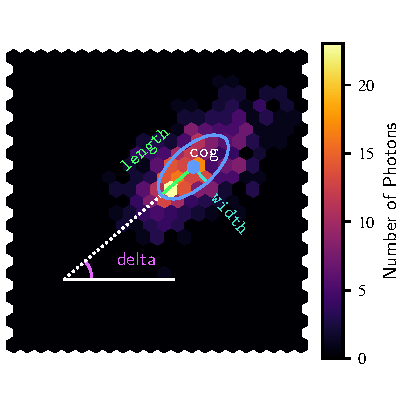
\includegraphics[width=0.7\textwidth]{Plots/hillas.pdf}%
  \caption{A graphical representation of a typical air-shower image. The figure shows the number of photons per pixel of an air-shower. The dotted
  line represents the air-shower axis. It corresponds to the line minimising the
  sum of perpendicular angular distance, weighted by the number of photons per
  pixel. The standard deviations along this axis and the perpendicular axis are
  the two features called length and width. The centre of
  gravity (cog) of the air-shower image is the two dimensional weighted
  mean of all shower pixels.}%
  \label{fig:hillas}%
\end{figure}
%
The figure shows the number of photons per pixel of an air-shower. The dotted
line represents the air-shower axis. It corresponds to the line minimising the
sum of perpendicular angular distance, weighted by the number of photons per
pixel. The standard deviations along this axis and the perpendicular axis are
the two features called \textbf{length} and \textbf{width}. The centre of
gravity (\textbf{cog}) of the air-shower image is the two dimensional weighted
mean of all shower pixels. The position and orientation of the shower is also
characterized by the angle \textbf{delta}. It is the angle between the shower
axis and the camera's $x$-axis. The \textbf{size} of the air-shower simply
corresponds to the sum of photons measured in all air-shower pixels.

To further parametrize the air-showers also higher order statistical moments of
the light distributions are used. Those are the third (\textbf{skewness}) and
fourth (\textbf{kurtosis}) statistical moments of the air-shower photons along
the two axes defined above. The values are calculated in a rotated system in
respective to the camera system, so that the two main axes define the
coordinate axes.
%
\begin{align}
  \text{skew}(X) &= \text{E}\left[\left(\frac{X-\mu}{\sigma}\right)^3\right] \label{eq:skew} \\
  \text{kurt}(X) &= \text{E}\left[\left(\frac{X-\mu}{\sigma}\right)^4\right]  \label{eq:kurt}
\end{align}
%
Additional to the size of an air-shower the \textbf{number of pixels}
containing air-shower photons is used as a feature.
%
\section{Reconstruction of the Source Position}
%
FACT is a single telescope and therefore has no stereoscopic features to
determine the origin of the cosmic ray showers. Thus, specific techniques only
using the features of the air-shower images have to be performed. In this
analysis the so called disp-method is used. It estimates the origin position of
the cosmic gamma-rays by calculating the disp and estimating the sign. The two
dimensional problem of determining $x$ and $y$ coordinates is turned into a
regression task and a classification task. The estimated source position within
the camera's image is assumed to be on the shower's main axis. To find this
position the first step is to estimate the distance to the cog of the
air-shower. disp is representing that distance of the estimated source inside
the camera. As described earlier the fraction of width and length is dependant
on the angle under that the air-shower is hitting the camera. Thus, it is
"pointing" to the cosmic origin of the shower. To estimate disp
\textbf{[FORMULA]}. The second step is to determine the direction of disp along
the main axis. As shown in \autoref{fig:disp_amb} the distance disp alone is
not sufficient to determine the source position, but an additional direction is
needed. Otherwise there remained an ambiguity, as shown in the two examples.
The assumption of the origin position being on the shower axis reduces this
task to a binary classification of the sign of disp.
%
\begin{figure}
  \begin{subfigure}{0.5\textwidth}
    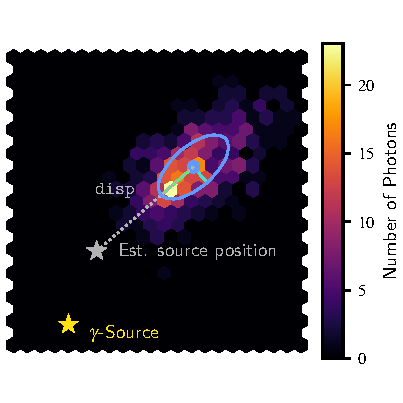
\includegraphics[width=\textwidth]{Plots/hillas_4.pdf}
  \end{subfigure}
  \begin{subfigure}{0.5\textwidth}
    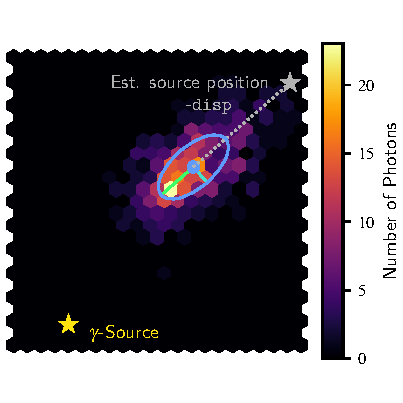
\includegraphics[width=\textwidth]{Plots/hillas_5.pdf}
  \end{subfigure}
  \caption{Disp method ambiguity.}
  \label{fig:disp_amb}
\end{figure}

%
\begin{figure}
  \centering%
  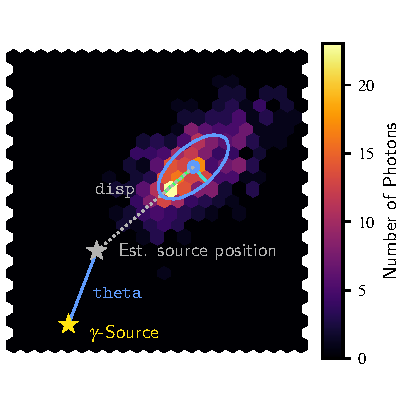
\includegraphics[width=0.67\textwidth]{Plots/hillas_disp.pdf}%
  \caption{Disp method.}%
  \label{fig:disp}%
\end{figure}
%
\section{Image Cleaning with pixelbased Thresholds}
%
When using the largest pulse representation (LP), there is a different cleaning
used. Since the PhotonStream is a different representation, of course the
optimal cleaning differs. When cleaning LP data an algorithm working on the PE
of the pixels is used. This cleaning is based on the assumption that air-shower
images contain a certain minimum number of photons per pixel and appear in a
quite small range of time and space within one event. It does not contain any
assumptions on the number of clusters per event, but with the mentioned
assumptions generally implies a certain topology within the camera's
coordinates. Since arrival times in this representation are properties per
pixel the time correlation has to be given between neighboring pixels. The
algorithm executes the following steps [paper]:
%
\begin{enumerate}
  \item find pixels containing more photons than an upper threshold $t_1$ (5~p.e.)
  \item remove pixels with less than 2 neighbors above $t_1$
  \item add neighbors of remaining pixels that are above a lower threshold $t_2$ (2.5~p.e.)
  \item remove pixels that have less than 2 neighbors arriving in $\SI{5}{\nano\second}$ time window
  \item remove single pixels with less than 2 neighbors
  \item remove pixels that have less than 2 neighbors inside a $\SI{5}{\nano\second}$ time window
\end{enumerate}
%
The remaining pixels are considered to be the cleaned image. When projecting
the PhotonStream data into a camera image and calculating the mean arrival
times per pixel, this cleaning can equivalently be performed on PhotonStream
data.


\section{Energy Estimation}
%
RANDOM FORESTS!!!11!!!elf!

\section{Signal-Background Separation}
%
RANDOM FORESTS!!!11!!!elf!

\chapter{The FACT Open Crab Sample}
%

\chapter{Results and Performance}
%
\section{Performance of the PhotonStream on Simulations}
%
\section{Performance of the PhotonStream on Data}
%
\section{Evaluation of the image cleaning}
%
\section{Parameters of DBSCAN}
%
\section{Pixelbased Threshold Cleaning on the PhotonStream}
%

\chapter{Summary}
%

\chapter{Conclusion and Outlook}
%

% \input{content/05_results.tex}


\appendix
% Hier beginnt der Anhang, nummeriert in lateinischen Buchstaben
\chapter{Appendix A}

\begin{table}
  \centering%
  \begin{tabular}{l
                  c
                  c}
      \toprule
      {}    & Anzahl der Filter in den Dichtelagen  & Struktur der Dropout Lagen      \\
      \midrule
      Modell 0    & (1024, 512, 128, 64, 32)  & (0.5, 0.4, 0.4, 0.3, 0.2) \\
      Modell 1    & (1024, 512, 256, 128, 64, 32, 16)  & (0.5, 0.4, 0.4, 0.4, 0.2, 0.2, 0.1) \\
      Modell 2    & (512, 256, 128, 64, 32, 16)  & (0.4, 0.4, 0.3, 0.3, 0.2, 0.1) \\
      Modell 3    & (1024, 256, 64, 16)  & (0.6, 0.4, 0.2, 0.1) \\
      Modell 4    & (512, 128, 32)  & (0.5, 0.3, 0.1) \\
      \bottomrule
  \end{tabular}
  \caption{Getestete Grundstrukturen für die Netzarchitekturen der alternativen Methode. Das $n$-te Element der Tupel beschreibt jeweils die Filtergröße der $n$-ten Dichtelage. Selbiges gilt für die Dropout Lagen. Es folgt auf jede Dichtelage (abgesehen von der letzten Lage) eine Dropout Lage.}
  \label{tab:grid}
\end{table}
%


\backmatter
\printbibliography

\cleardoublepage
\thispagestyle{empty}
\section*{Eidesstattliche Versicherung}
Ich versichere hiermit an Eides statt, dass ich die vorliegende Abschlussarbeit mit dem Titel \enquote{\thetitle} selbstständig und ohne unzulässige fremde Hilfe erbracht habe.
Ich habe keine anderen als die angegebenen Quellen und Hilfsmittel benutzt, sowie wörtliche und sinngemäße Zitate kenntlich gemacht.
Die Arbeit hat in gleicher oder ähnlicher Form noch keiner Prüfungsbehörde vorgelegen.

\vspace*{1cm}\noindent
\begin{center}
  \begin{tabular}{@{}p{0.4\textwidth}@{\hspace{0.15\textwidth}}p{0.4\textwidth}@{}}
  \rule{\linewidth}{0.25pt}& \rule{\linewidth}{0.25pt}\\
  Ort, Datum & Unterschrift
  \end{tabular}
\end{center}

\subsection*{Belehrung}
Wer vorsätzlich gegen eine die Täuschung über Prüfungsleistungen betreffende Regelung einer Hochschulprüfungsordnung verstößt, handelt ordnungswidrig.
Die Ordnungswidrigkeit kann mit einer Geldbuße von bis zu \SI[round-mode=places, round-precision=2]{50000}{€} geahndet werden.
Zuständige Verwaltungsbehörde für die Verfolgung und Ahndung von Ordnungswidrigkeiten ist der Kanzler/die Kanzlerin der Technischen Universität Dortmund.

Im Falle eines mehrfachen oder sonstigen schwerwiegenden Täuschungsversuches kann der Prüfling zudem exmatrikuliert werden \mbox{(\S\,63 Abs. 5 Hochschulgesetz --HG--).}

Die Abgabe einer falschen Versicherung an Eides statt wird mit Freiheitsstrafe bis zu 3 Jahren oder mit Geldstrafe bestraft.

Die Technische Universität Dortmund wird ggf.\ elektronische Vergleichswerkzeuge (wie z.\,B.\ die Software \enquote{turnitin}) zur Überprüfung von Ordnungswidrigkeiten in Prüfungsverfahren nutzen. \\[\baselineskip]

\noindent Die oben stehende Belehrung habe ich zur Kenntnis genommen.\\[1cm]
\begin{center}
\begin{tabular}{@{}p{0.4\textwidth}@{\hspace{0.15\textwidth}}p{0.4\textwidth}@{}}
\rule{\linewidth}{0.25pt}& \rule{\linewidth}{0.25pt}\\
Ort, Datum & Unterschrift
\end{tabular}
\end{center}

\end{document}
